\documentclass[final-report]{report-template}

\usepackage{graphicx} % Required for inserting images
\usepackage[HTML]{xcolor}
\usepackage{amsmath} 
\usepackage{float}
\usepackage[section]{placeins}

\usepackage{verbatim}
\usepackage{hyperref}

\usepackage{amsmath}  % cases environment, \text, \dfrac
\usepackage{amssymb}  % \mathbb (for \mathbb{R})

\usepackage{tabularx}
\usepackage{booktabs}
\usepackage{graphicx}

% \graphicspath{{figures/}} configure a file path to save you typing it out everytime we want to load a figure

%python colours
\definecolor{pyblue}{HTML}{1F77B4}
\definecolor{pyorange}{HTML}{FF7F0E}
\definecolor{pygreen}{HTML}{2CA02C}
\definecolor{pyred}{HTML}{D62728}

% Metadata used for the title page - please modify.
\university{Imperial College London}
\department{Department of Earth Science and Engineering}
\course{MSc in Environmental Data Science and Machine Learning}
\title{Solving Inverse Problems in Bio-Physics Using Neural Physics}
\author{Ishan Mitra}
\email{imitra694@gmail.com}
\githubusername{ishan4589}
\supervisors{Dr Claire Heaney\\
             Professor Christopher Pain}

\begin{document}

\maketitlepage  % generate title page

%TC:ignore
\textbf{AI Declaration}:

I used Anthropic’s Claude Opus 5 (https://claude.ai/) for help with the implementation of the multigrid solver, the distorted grid, and plotting visualisations. I used it to help refactor the codebase to move functionality outside of Jupyter Notebooks into Python scripts and write tests for my code. I also used Claude to help understand the theory required to distort the grid and the relevant biophysics technical knowledge needed for this project. I used OpenAI’s ChatGPT 5.6 (https://chat.openai.com/) to verify docstrings and comments in my repository were correct. All AI-generative tools helped my learning and understanding and I declare that all of the submitted work reflects my own understanding, decisions, and contributions as declared in the Academic Integrity Declaration.
%TC:endignore

\section{Abstract}

Using Surface electromyography (sEMG) readings offers a non-invasive way of monitoring muscle health by inferring the electrical conductivities of underlying tissues. However, recovering these parameters from surface measurements is challenging. This paper applies the Neural Physics approach of Chen et al.~\cite{chen2026}, which provides a differentiable solver that is very useful for inverse problems. We first solve the forward problem to generate synthetic sEMG measurements from prescribed ground-truth tissue conductivities and tissue geometry, which are our parameters. In the inverse problem, we then attempt to iteratively update estimates of these quantities to minimise the misfit between the synthetic data and the data predicted by the model.

\section{Problem Description}

In this problem, we attempt to use surface electromyography results, which are obtained by electrodes placed on the surface of the skin, to obtain the underlying geometry and conductivities of bone, muscle, fat and skin tissue layers.

\subsection{Significance}

The study of electrical activity within muscle cells, muscle electrophysiology, is a critical area when assessing muscle health. We prefer to avoid invasive procedures that can involve breaking the skin barrier, as they increase recovery time and introduce the risk of complications. This motivates the following inverse problem; given sEMG readings which are taken non-invasively, we try to figure out key information about the limb, such as the underlying tissue conductivities and geometry. Reliably recovering the parameters this way could provide important information about muscle health, while circumnavigating the need for invasive procedures.

\subsection{Literature review}

We can use solutions of the Maxwell's equations to obtain properties of tissue conductivity. Surface electromyography uses surface electrodes applied directly to the skin, to detect and record the electrical activity produced by muscle fibres. The low frequencies of signal sources that we read from the electrodes allow us to ignore the physical effects which couple electricity to magnetism. This allows us to apply the quasi-static assumption to the Maxwell equations ~\cite{plonsey1977}, ~\cite{plonsey1967} and our sEMG volume-conductor forward problem reduces to a Poisson partial differential equation.~\cite{mesin2013} We apply a homogeneous Neumann boundary condition to reflect our assumption that the skin-air interface is the insulating boundary, so no current flows between the skin and air. Hence, we arrive at the following equation:~\cite{maksymenko2023}:

$$
\begin{cases}
\nabla \cdot (\sigma \nabla \phi) = -I & \text{in } \Omega \\
\sigma \dfrac{\partial \phi}{\partial \mathbf{n}}
  = \sigma \nabla \phi \cdot \mathbf{n} = 0 & \text{on } \partial \Omega
\end{cases}
$$

where, \newline
$\Omega \subset \mathbb{R}^3$ is a volume conductor domain of interest, \newline$\partial \Omega$ is the boundary of the volume conductor boundary, \newline $\mathbf{n}$ is the outward pointing normal unit vector, \newline $\phi(\mathbf{x})[V]$ is the electric potential we measure at the surface electrodes, \newline $I(\mathbf{x})[A/m^3]$ is the current source density, \newline $\sigma(\mathbf{x})[S/m]$ is the conductivity.

We interpret the current source density $I(\mathbf{x})$ as the current density entering or leaving the extracellular medium at position $\mathbf{x} \in \Omega$. A source or a sink is determined from the perspective of the tissue surrounding the muscle fibre, where a negative value for $I$ indicates a sink, so the current is leaving the extracellular medium and a positive value indicates the opposite.~\cite{nicholson1975},~\cite{pettersen2012}

In this paper, we use a cylindrical volume conductor model, where we assume the medium to be piecewise-homogeneous in which concentric shells represent tissue layers for the skin, fat, muscle and bone. The handling of the tissue interfaces is outlined in section ~\ref{sec:tissue-interface}. We assign plausible ground truth conductivity values for each layer ~\cite{farina2004}, where the muscle is assumed to be anisotropic figure~\ref{fig:radial-conductivity-profile}. Subcutaneous tissue is assumed to have variable thickness~\cite{mesin2013}, so the thickness of the skin is fixed. Assuming tissue layers to be clinically variable quantities results in their interface radii entering the parameter vector we recover. Kolehmainen et al~\cite{kolehmainen1999} solve this class of problem for general elliptic PDEs with assumed, known, underlying coefficient values. Here we recover both. Therefore, we believe this paper's novelty lies in the use of the Neural Physics approach ~\cite{chen2026} to solve for the potential field $\phi$ sampled at the surface electrodes, which we then use to tackle the inverse problem of jointly retrieving the conductivities and tissue geometry.

\subsection{Objectives}

This area of research requires ground-truth for the current source density and conductivity. However, these parameters can be challenging to obtain in real life. Therefore, our first objective is the forward problem, which involves generating realistic, synthetic EMG readings from ground truth parameters we set manually. This motivates our second objective; the inversion step, where we iteratively improve our guess for the underlying conductivity and thickness of the tissue layers by minimising a data misfit function, to retrieve the underlying geometry and conductivity from surface electrode readings alone. We will aim to get less than 10\% relative error on all parameters while maintaining about 9\% random measurement error at the electrodes.

\begin{figure}[H]
  \centering
  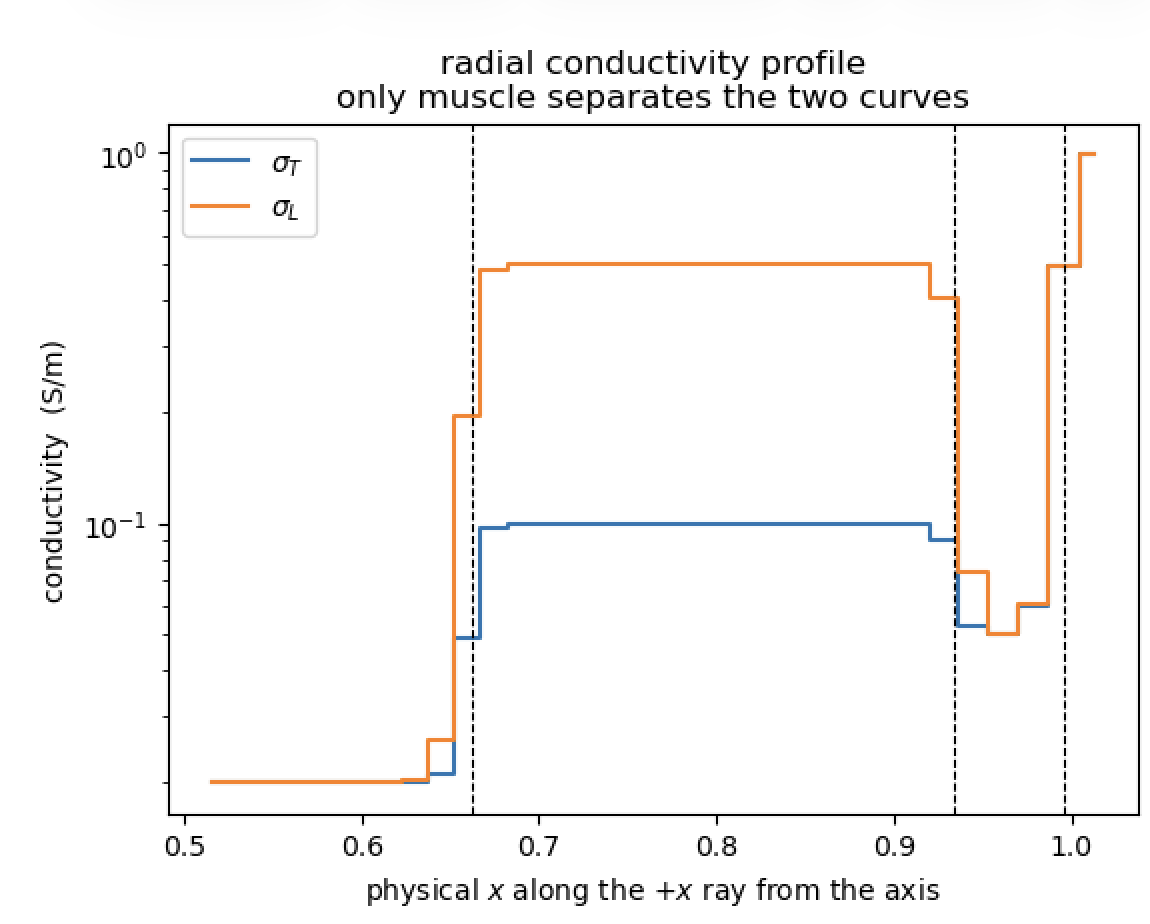
\includegraphics[width=0.8\linewidth]{experiment-design-figures/radial-conductivity-profile.png}
  \caption{Anisotropy in the muscle layer as we traverse the cross section of the limb.}
  \label{fig:radial-conductivity-profile}
\end{figure}

\newpage

\section{Methodology}

\subsection{Workflow}

Our governing equation
$$\nabla \cdot (\sigma \nabla \phi) = -I$$
can be discretised as follows,
$$A(\sigma) \phi = -I,$$

where $A(\sigma)$ becomes our discrete operator for the quasi-static Maxwell equation. We will outline how we handle the discretisation in Section~\ref{sec:operator-discretisation}. However, as previously outlined in this paper, we will invert for the tissue conductivities $\boldsymbol{\sigma}$ and the tissue interface radii $R$, so the radii enter the operator as the locations where the conductivity field jumps due to our piecewise-homogeneity assumption. Hence, our ground-truth parameter vector becomes $\theta_{\text{true}} = (\boldsymbol{\sigma_{\text{true}}}, R_{\text{true}})$, which is used in the forward solve to generate synthetic data $\phi_{\text{obs}}$. We do not recover the current source density term $I$, hence, it is fixed and known throughout the data generation and inversion step. Writing the operator as a function of our full parameter vector $\theta$ yields the following discrete system,

$$
A(\theta_{\text{true}})\phi_{\text{true}} = -I,
$$
where the forward solve is a linear in $\phi$ for fixed $\theta$.

It is crucial to note that our operator $A(\theta)$ is singular due to the homogeneous Neumann boundary condition. This determines the electric potential $\phi$ only up to an additive constant, and the system admits a solution only for sources $I$ which have zero net current. We detail how we deal with these in Sections ~\ref{sec:neumann} and ~\ref{sec:source-initialisation}.

We then sample $\phi_{\text{true}}$ using surface electrodes placed on the skin
surface and add measurement noise, to obtain our synthetic measurements

$$
\phi_{\text{obs}} = M\phi_{\text{true}} + \eta,
$$

where $M$ selects the electrode nodes and $\eta$ is the measurement noise. In the forward solve, we use a multigrid method to compute $\phi$, due to its computational efficiency~\cite{chen2026} and ability to remove low frequency errors.

The inverse problem can be formulated as the following parameter-to-solution map,

$$
\theta \;\longmapsto\; M\phi(\theta),
\qquad
\text{where } A(\theta)\phi(\theta)=-I.
$$


As we can see the map from $\theta$ to $\phi$ is non-linear, due to the operator's dependence on $\theta$.

The recovery of $\theta$ does not admit a close form solution, so we obtain it by iteratively minimising a loss function. This requires derivatives of a data misfit objective function with respect to $\theta$, which highlights our motivation for the following workflow. We initialise a guess for our parameter vector $\hat{\theta}$, and use it to compute predicted surface electrode readings $\phi_{\text{pred}}$ in the forward solve i.e. $A(\hat{\theta})\phi_{\text{pred}} = -I$. We then attempt to minimise the following data misfit between our observed and predicted electric potential,

$$
L(\hat\theta) = \frac{1}{2}\bigl\lVert \phi_{\text{obs}} - \phi_{\text{pred}}(\hat\theta) \bigr\rVert_2^2\Big|_{M}
$$

to update our guess for $\hat{\theta}$ using the gradient $\partial L / \partial \hat{\theta}$.

So the method consists of an outer loop which iteratively updates the parameter $\theta$ using the L-BFGS-B algorithm, and the the inner loop uses a V-cycle multigrid solver to compute our predicted data $\phi_{\text{pred}}$. In practice, we assemble our discrete operator $A(\theta)$ as convolutional layers with analytically determined weights, which are not updated via training, as outlined in the Neural Physics approach ~\cite{chen2026}. This method offers complete differentiability, which makes our inverse problem tractable. The gradient is available because every operation in the solve is a PyTorch tensor operation with a defined derivative. Reverse-mode differentiation therefore, propagates gradients through the solver~\cite{paszke2019}.

\subsection{Tissue interfaces}
\label{sec:tissue-interface}

Due to our earlier assumption of the tissue layers being represented as concentric shells on the axis of the limb $(x_c, y_c)$, we write $r((x, y)) = \lVert (x - x_c,\, y - y_c) \rVert$ for the transverse distance from the axis. Our layers become; bone, $0 \le r < R_1$, muscle, $R_1 \le r < R_2$, fat, $R_2 \le r < R_3$, skin, $R_3 \le r < R_4$, $R_4$ being the outermost radius of the limb, which is where the insulating boundary condition is imposed. We assume the following numbers for the interface radii; $R_1=7\,\mathrm{mm}$, $R_2=20\,\mathrm{mm}$, $R_3=23\,\mathrm{mm}$ and $R_4=24\,\mathrm{mm}$ ~\cite{maksymenko2023}.

Since the thickness of the bone, muscle, and fat layers are clinically variable quantities in our experiment, we will attempt to recover them. The thickness of the skin is modelled as a known quantity of $1\,\mathrm{mm}$, hence, the outermost interface $R_3 = 23\,\mathrm{mm}$ is a fixed constant. The three inner layers therefore partition $[0, R_3]$ and their thicknesses satisfy
$$
R_1 + (R_2 - R_1) + (R_3 - R_2) \;=\; R_3 \;=\; 23\,\mathrm{mm},
$$
so $R_1$ and $R_2$ completely determine $R_3$, therefore,  we only need to invert for $R_1$ and $R_2$.


In this paper, rather than having tissue layers meet at sharp boundaries, we model them as
gradually transitioning into one another, following the diffuse-interface
approach of~\cite{li2009}. This is a natural choice because we want the conductivity to remain differentiable in the interface radii, which would not be possible with hard boundaries.

Since $0 < R_1 < R_2 < R_3$ are the interface radii, ordered outwards, and we let $\sigma_0, \sigma_1, \sigma_2, \sigma_3$ be the conductivities of the tissue layers they separate. Note we only consider four conductivities here, because tissue interfaces only exist in the transverse plane, which is the cross-section of the limb, hence, in this section we do not account for muscle's conductivity in the longitudinal direction, which is along the muscle fibre. We will write
$$
L(t) \;=\; \frac{1}{1 + e^{-t}}
$$
for the logistic function and set
$$
s_k(r) \;=\; L\!\left(\frac{r - R_k}{\varepsilon}\right),
\qquad k = 1, 2, 3 ,
$$
with a transition width $\varepsilon$ shared by all three, so that $s_k$ rises from $0$ to $1$ across a band of width $\mathcal O(\varepsilon)$ centred on $r = R_k$.

The tissue layers are assigned the following weights,
$$
w_0 = 1 - s_1, \qquad
w_1 = s_1 - s_2, \qquad
w_2 = s_2 - s_3, \qquad
w_3 = s_3.
$$
They are the differences between the two interfaces bounding each layer, so that $\sum_{k=0}^{3} w_k = 1$ holds identically. 

$L$ is a monotone function and since $R_{k+1} > R_{k}$, we have that $s_k \ge s_{k+1}$, so $w_k \ge 0$ for every $k$. The smoothed conductivity, $\sigma_\varepsilon(r) = \sum_{k=0}^{3} \sigma_k \, w_k(r)$, is a weighted average of the four layer values, hence, it lies between the smallest and largest of them for every $\varepsilon > 0$. It can never become negative by construction, because $\sigma_k > 0$ for every $k$.

We regroup by $s_k$ to obtain,
$$
\sigma_\varepsilon \;=\; \sigma_0 + \sum_{k=1}^{3} (\sigma_k - \sigma_{k-1}) \, s_k ,
$$
where every $s_k$ appears once and is weighted by the conductivity jump it carries. The hard boundary model says that each $s_k$ is a step, whereas, the smoothed model replaces each step by a smooth transition. For every $\varepsilon > 0$, the conductivity is smooth instead of piecewise constant; true piecewise homogeneity is recovered only in the limit $\varepsilon \to 0^{+}$ (cf.~\cite{burger2017}).

\subsection{Grid Construction}

We use the following stretching map to project our square onto a disc, as outlined by Fanxin Sun's approach to this problem ~\cite{Sun2025}. Our function uses a radial rescaling based on the ratio of two different norms.

We use a vertex-centred grid with \(n_x\) and \(n_y\) physical nodes and a one-node halo on each side. These extra nodes are needed to calculate centred differences at the boundary, so the haloed coordinates are indexed, \(i=0,\ldots,n_x+1\) and \(j=0,\ldots,n_y+1\), with $x_i=i\,\Delta x$ and $y_j=j\,\Delta y.$

The physical grid occupies $i=1,\ldots,n_x$ and $j=1,\ldots,n_y$. Its centre is

$$
o_x=\frac{1}{2}(n_x+1)\Delta x,
\qquad
o_y=\frac{1}{2}(n_y+1)\Delta y,
$$

and we work in coordinates measured from that centre,

$$
u=x-o_x,
\qquad
v=y-o_y.
$$


Each node admits the following two radii: the Euclidean radius $r = \sqrt{u^2+v^2}$, whose level sets are circles, and the max-norm radius $s = \max(|u|,|v|)$, whose level sets are squares. Since $s^2 = \max(u^2,v^2) \le u^2 + v^2 = r^2$, we have that $s \le r$, with equality only on the axes.

Our map moves each node along its own ray from the centre, but leaves its direction unchanged. This sends the square of max-norm radius $s$ onto the circle of Euclidean radius $s$. This map has the form $(u,v) \mapsto \alpha\,(u,v)$, where $\alpha$ is a positive scalar, and the mapped point has Euclidean radius $\alpha r$.
\[
  \alpha = \frac{s}{r}, \qquad
  x' = \alpha u + o_x, \qquad
  y' = \alpha v + o_y.
\]

Because $s \le r$ we always have $\alpha \le 1$, so every node moves inward. Figure~\ref{fig:square-to-disc} offers a visual demonstration of this. On the axes, where $v = 0$ or $u = 0$, we have $s = r$ and $\alpha = 1$, so the nodes do not change position. However, on the diagonals, where $|u| = |v|$, we have $s = |u|$ and $r = \sqrt{2}\,|u|$, giving $\alpha = 1/\sqrt{2}$, which is where the greatest compression occurs. Therefore, nodes end up clustered near the diagonals and stretched thin near the axes. This uneven compression motivates the need for Laplacian mesh smoothing which we introduce below. Note that $\alpha$ is undefined at $r = 0$, so the centre node is fixed by definition.

Another drawback of this raw projection map is that its not continuously differentiable ($C^1$), it is only continuos ($C^0$) because $\max(|u|,|v|)$ is not differentiable where $|u|=|v|$, which are the two diagonals of the reference square. We highlight the accuracy cost of this in Figure~\ref{fig:seam-error}.

\begin{figure}[H]
  \centering
  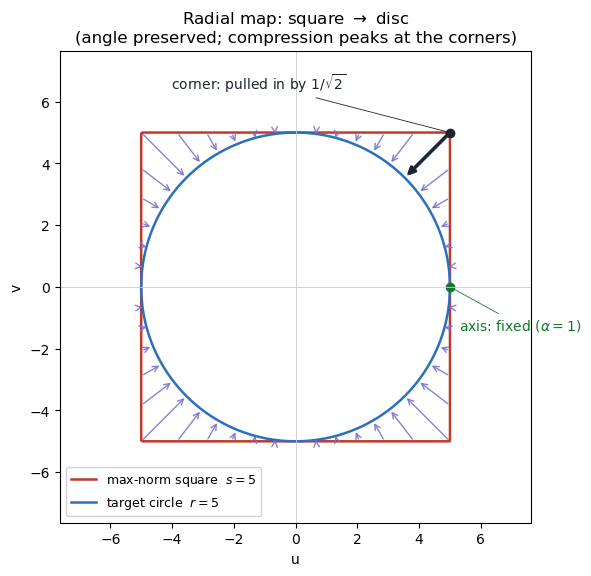
\includegraphics[width=0.8\linewidth]{experiment-design-figures/square-disc-visualisation.png}
  \caption{Visualising the grid distortion.}
  \label{fig:square-to-disc}
\end{figure}

We relax the mesh using the diffusion equation, which drives the coordinate fields towards a steady state,

$$
\frac{\partial q}{\partial t}=\nabla^2q,
\qquad q\in\{x,y\}.
$$

The $x$- and $y$-coordinate fields are smoothed independently and simultaneously over unit-spaced grid-index space, while the outer-ring coordinates remain fixed. The five-point Laplacian is approximated by

$$
\nabla^2q\approx
q_{i+1,j}+q_{i-1,j}+q_{i,j+1}+q_{i,j-1}-4q_{i,j},
$$

which gives the Jacobi update,

$$
q_{i,j}^{(k+1)}=q_{i,j}^{(k)}
+\omega\left(
q_{i+1,j}^{(k)}+q_{i-1,j}^{(k)}
+q_{i,j+1}^{(k)}+q_{i,j-1}^{(k)}
-4q_{i,j}^{(k)}\right).
$$

We use $\omega=0.2$, so each node moves towards the neighbour average while retaining one-fifth of its previous position. We apply $100$ iterations, which tends toward a discrete harmonic placement which smooths the node spacing but does not make uniform.


\begin{figure}[H]
  \centering
  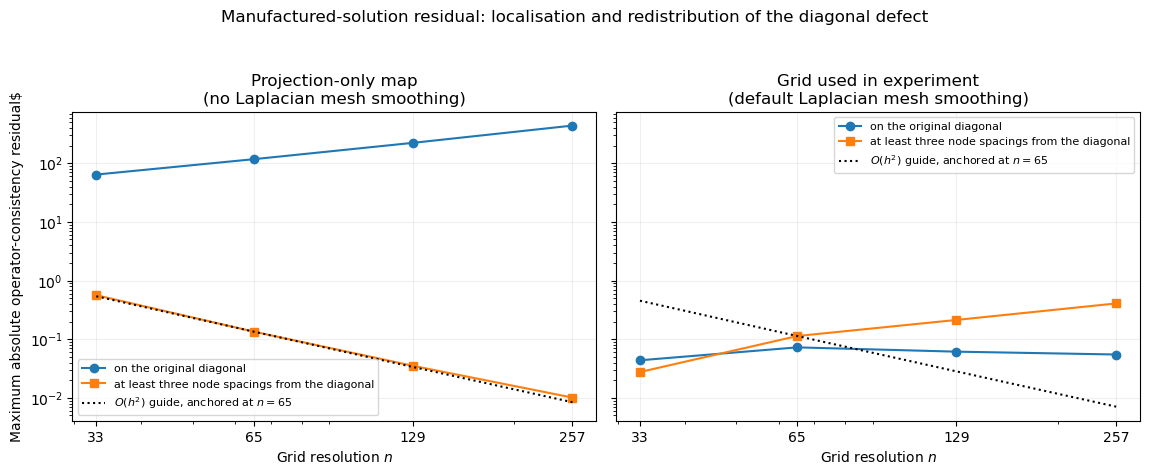
\includegraphics[width=0.8\linewidth]{experiment-design-figures/seam-error.png}
  \caption{Effects of mesh smoothing on the manufactured-solution residual near the diagonal seams.}
  \label{fig:seam-error}
\end{figure}

The above figure\ref{fig:seam-error} indicates that the projection-only map exhibits inconsistent behaviour on the non-differentiable diagonals. The residuals outside the diagonal band decay at approximately second order, $\mathcal{O}(h^2)$, whereas the residual on the diagonal grows as the grid resolution increases. As we can see the mesh smoothing reduced the peak residual on the original diagonal by several orders of magnitude, evidenced by the blue curve in the second graph sitting much lower than in the first one and that it is no longer increasing. Nevertheless, the smoothing procedure does not solve the whole problem because it transfers the defect into neighbouring grid layers, as shown by the orange curve steadily increasing with resolution in the second graph, instead of decreasing as it did before. Hence, this figure demonstrates that smoothing cannot remove the accuracy limitation inherited from the non-differentiable mapping.


\subsection{PDE Transformation}
\label{sec:general-map}

We will solve our physical equation $\nabla_x\cdot(\sigma\nabla_x\phi)=-I$ on a 3D structured grid with coordinates $\xi=(\xi,\eta,\zeta)$. The map $x=\Phi(\xi)$ will carry the geometry, where $x=(x,y,z)$ are the physical coordinates on the distorted, cylindrical grid. $J_{ij}=\partial x_i/\partial\xi_j$.So $J=\partial(x,y,z)/\partial(\xi,\eta,\zeta)$ is fixed by convention.

For a scalar field $\phi: \mathbb{R}^3 \rightarrow \mathbb{R}$, we have via the chain rule,

$$
\frac{\partial\phi}{\partial\xi_j}=\sum_i\frac{\partial\phi}{\partial x_i}\frac{\partial x_i}{\partial\xi_j}=\sum_i J_{ij}\,(\nabla_x\phi)_i
\;\Longrightarrow\; \nabla_\xi\phi=J^{\mathsf T}\nabla_x\phi
\;\Longrightarrow\; \nabla_x\phi=J^{-\mathsf T}\nabla_\xi\phi .
$$

We let $\Phi$ be a smooth, invertible mapping with $\mathcal J=\det J>0$ everywhere, so that $J^{-1}$ exists. This yields the identity below, where the derivation is deferred to the appendix~\ref{sec:strong-form-derivation}:

$$
\;\nabla_x\!\cdot(\sigma\nabla_x\phi)=\frac{1}{\mathcal J}\,\nabla_\xi\!\cdot(\tilde\sigma\nabla_\xi\phi)
$$

We can then multiply the above equation by $\mathcal J$ and substitute in the quasi-static Maxwell equation to obtain,

$$
\nabla_\xi\!\cdot(\tilde\sigma\,\nabla_\xi\phi)=-\mathcal J\,I ,
$$

which puts the weight onto the source term and leaves the operator as a divergence of a flux $\tilde\sigma\nabla_\xi\phi$.

We take our cylindrical grid to be straight extrusion, obtained by stacking circular cross-sections along the longitudinal z axis. Hence, $x,y$ depend only on $(\xi,\eta)$ and $z=z(\zeta)$, and we can take $J$ to be block-diagonal:

$$
J=\begin{pmatrix}J_2 & 0\\ 0 & z_\zeta\end{pmatrix},
\qquad
J_2=\frac{\partial(x,y)}{\partial(\xi,\eta)}=\begin{pmatrix}a & b\\ c & d\end{pmatrix},
\qquad
\mathcal J=\det(J_2)\,z_\zeta,
$$

with $a=x_\xi,\ b=x_\eta,\ c=y_\xi,\ d=y_\eta$ and $z_\zeta$ is constant.

Our conductivity tensor $\sigma=\operatorname{diag}\big(\sigma_T,\sigma_T,\sigma_L\big)$ can be written in block-form,


$$
\sigma=\begin{pmatrix}\sigma_T I_2 & 0\\ 0 & \sigma_L\end{pmatrix}.
$$

The transform respects the blocks and yields the following result, where the derivation is handled in the appendix~\ref{sec:transformed-conductivity-derivation}:

$$
\tilde\sigma=\sigma_T\,(M_T\oplus 0)\;+\;\sigma_L\,(0\oplus m_L)
=\begin{pmatrix}\sigma_T m_{xx}&\sigma_T m_{xy}&0\\ \sigma_T m_{xy}&\sigma_T m_{yy}&0\\ 0&0&\sigma_L m_L\end{pmatrix}.
$$

where $M_T = \begin{pmatrix} m_{xx} & m_{xy}\\ m_{xy} & m_{yy} \end{pmatrix} = \frac{z_\zeta}{\det J_2} \begin{pmatrix} b^2+d^2 & -(ab+cd)\\ -(ab+cd) & a^2+c^2 \end{pmatrix}$ and $m_L=\frac{\det J_2}{z_\zeta}$ represents the in-plane compression.

The tensor $\tilde\sigma (x)$ applies pointwise at every node $x$. Our operator takes the entries of $\tilde\sigma$ to encode the geometry of the physical grid. By feeding these terms into the operator, we are able to use uniform-cube finite differences and our geometric multigrid solver, which are intended for a regular grid, to solve on the curved cylinder.

As we can see the mesh distortion introduces the cross-term $m_{xy}$ into the conductivity tensor. It is important to be aware that $m_{xy}$ does not appear due to diagonally oriented muscle fibres because we take them to be aligned with the physical  $z$-axis, which is why our physical space conductivity $\sigma$ is diagonal.

\subsection{Discretisation of the operator}
\label{sec:operator-discretisation}

Since the coordinate transformation has been outlined, we can now discretise the following operator, in computational coordinates $\nabla_\xi\!\cdot(\tilde\sigma\,\nabla_\xi\phi)$.

We consider one spatial dimension in the derivation because the axes are independent. We take one axis with a variable coefficient $a$ and let $F=a\,\partial_\xi\phi$ be the flux, so we have $L\phi=\partial_\xi\!\left(a\,\partial_\xi\phi\right)=\partial_\xi F$. The scheme uses two centred-differences on two different grids.

First we tackle the outer derivative, where the two face midpoints either side of node $i$ sit at $i\pm\tfrac12$, a distance $h$ apart and symmetric about the node,

$$
\big(\partial_\xi F\big)_i \approx \frac{F_{i+\frac12}-F_{i-\frac12}}{h}.
$$

Now we tackle the inner derivative, where the two nodes $i$ and $i+1$ sandwich the face midpoint at $i+\tfrac12$,

$$
F_{i+\frac12} \approx a_{i+\frac12}\,\frac{\phi_{i+1}-\phi_i}{h}.
$$

Both differences are centred about their own evaluation point. We now substitute the second expression into the first to obtain,

$$
(L\phi)_i=\frac{1}{h}\left[a_{i+\frac12}\,\frac{\phi_{i+1}-\phi_i}{h}
-a_{i-\frac12}\,\frac{\phi_i-\phi_{i-1}}{h}\right]
=\frac{a_{i+\frac12}\phi_{i+1}-\big(a_{i+\frac12}+a_{i-\frac12}\big)\phi_i+a_{i-\frac12}\phi_{i-1}}{h^2}.
$$

In each coordinate direction, the face coefficient combines the relevant conductivity component with its corresponding term that encodes the geometry:

$$
a^{(\xi)}_{i+\frac12} = \big(\sigma_T\, m_{xx}\big)_{i+\frac12}, \qquad
a^{(\eta)}_{j+\frac12} = \big(\sigma_T\, m_{yy}\big)_{j+\frac12}, \qquad
a^{(\zeta)}_{k+\frac12} = \big(\sigma_L\, m_L\big)_{k+\frac12}.
$$

Each face value is built from the two nodes either side and the full coefficients $\sigma m$ are averaged onto the faces harmonically i.e. $a_{i + \frac{1}{2}}$ = harm$((\sigma m)_i, (\sigma m)_i)$, which we will derive in the next Section~\ref{sec:averaging-face-coefficients}.

The cross term cannot be made into a two point face-flux. This is because on a $\xi$-face the flux component is $\sigma_T\big(m_{xx}\phi_\xi+m_{xy}\phi_\eta\big)$, so the second part is a derivative along the face of a node's control volume. We therefore, discretise this by using the midpoint rule at each cell centre, the full derivation is given in appendix~\ref{sec:cross-term}. Since, this is a cell-centred midpoint rule instead of a two-point face-flux, there is no reason to use a harmonic mean to encode the transmission condition like before. Hence, the cell-centred coefficient is obtained by an arithmetic average of the four corner values of the $\sigma_Tm_{xy}$ term.

\subsection{The Homogeneous Neumann Boundary Condition}
\label{sec:neumann}

Consider our mapped flux $\mathbf F = \tilde\sigma\,\nabla_\xi\phi$, where $\nabla_\xi\cdot\mathbf F = -\mathcal J I$ holds due to the derivation in Section~\ref{sec:general-map}. We integrate $\nabla_\xi\cdot\mathbf F$ over $V_{ijk}$ and applying the divergence theorem to yield the following,

$$
\sum_{f \subset \partial V_{ijk}} \int_f \mathbf F\cdot\mathbf N\,\mathrm{d}S
\;=\; -\int_{V_{ijk}} \mathcal J I \,\mathrm{d}\xi .
$$

We can now split the surface, where an interior node, $\partial V_{ijk}$ consists entirely of faces shared with neighbouring control volumes and for a boundary node, part of $\partial V_{ijk}$ lies on
$\partial\Omega$, where the control volume's outward normal is the domain's outward
normal.

$$
\underbrace{\sum_{f \subset \Gamma^{\text{int}}_{ijk}} \int_f \mathbf F\cdot\mathbf N\,\mathrm{d}S}_{\text{unknown, must be discretised}}
\;+\;
\underbrace{\int_{\Gamma^{\text{bd}}_{ijk}} \mathbf F\cdot\mathbf N\,\mathrm{d}S}_{=\;0\ \text{by the boundary condition}}
\;=\; -\int_{V_{ijk}} \mathcal J I \,\mathrm{d}\xi .
$$

Since the second term vanishes due to the insulating boundary condition, we impose this by dropping those faces from the sum, so all that remains are the interior-face integrals, which we discretise as usual.

For any differentiable $\phi$ and any $c \in \mathbb{R}$, $\nabla_\xi(\phi + c) = \nabla_\xi\phi$. Hence

$$\nabla_\xi \cdot \big(\tilde\sigma \nabla_\xi(\phi + c)\big) = \nabla_\xi \cdot (\tilde\sigma \nabla_\xi\phi) = -\mathcal{J} I,$$
$$\mathbf{N} \cdot \big(\tilde\sigma \nabla_\xi(\phi + c)\big) = \mathbf{N} \cdot (\tilde\sigma \nabla_\xi\phi) = 0,$$

so the solution $\phi$ is only determined up to an additive constant. Hence, our discrete operator $A(\theta)$ is singular because it has a non-zero right null space, so to obtain a unique solution, we impose a zero-sum constraint~\cite{maksymenko2023} on the potentials $\phi$. The implications of the insulating boundary condition on the source term are outlined in Section \ref{sec:source-initialisation}.

\subsection{Creating the current source density}
\label{sec:source-initialisation}

In our approach, we adapt the practice of separating the signals from individual motor units and recovering their electric potential readings individually~\cite{delvecchio2020}. We apply this to our method by treating our sources as two separate measurements. Each electric potential pattern is a response to a single source $s$ within the muscle layer, hence, two sources at varying depths return two distinct measurements of the same tissue, instead of one combined recording.

For each source $s$, the potential field is obtained from the separate forward solve,
$$
A(\theta)\phi_s=b_s.
$$

Let $m$ denote the number of nodes retained by the surface measurement mask. We define the forward map more rigorously, by stacking the masked potential fields from the two sources:
$$
F:\mathbb{R}^7\longrightarrow\mathbb{R}^{2m},
\qquad
F(\theta)=\bigl[\phi_s(\theta)\bigr]_{s,\mathrm{mask}}.
$$

The tissue layers have a concentric shell structure, whose only variation is due to changes in depth. This means that a rotation of the source around the axis would give rise to a rotated version of the same data field and provide no additional information. However, a change in the source's depth will change the way its data field interacts with the tissue boundaries. Hence, we initialise the two sources at different interface radii.

To initialise the sources we use a fixed dipole model~\cite{malmivuo1995}, which involves placing a dipole at a given location. We simulate the dipoles by using a Gaussian distribution to generate them.

\begin{figure}[H]
  \centering
  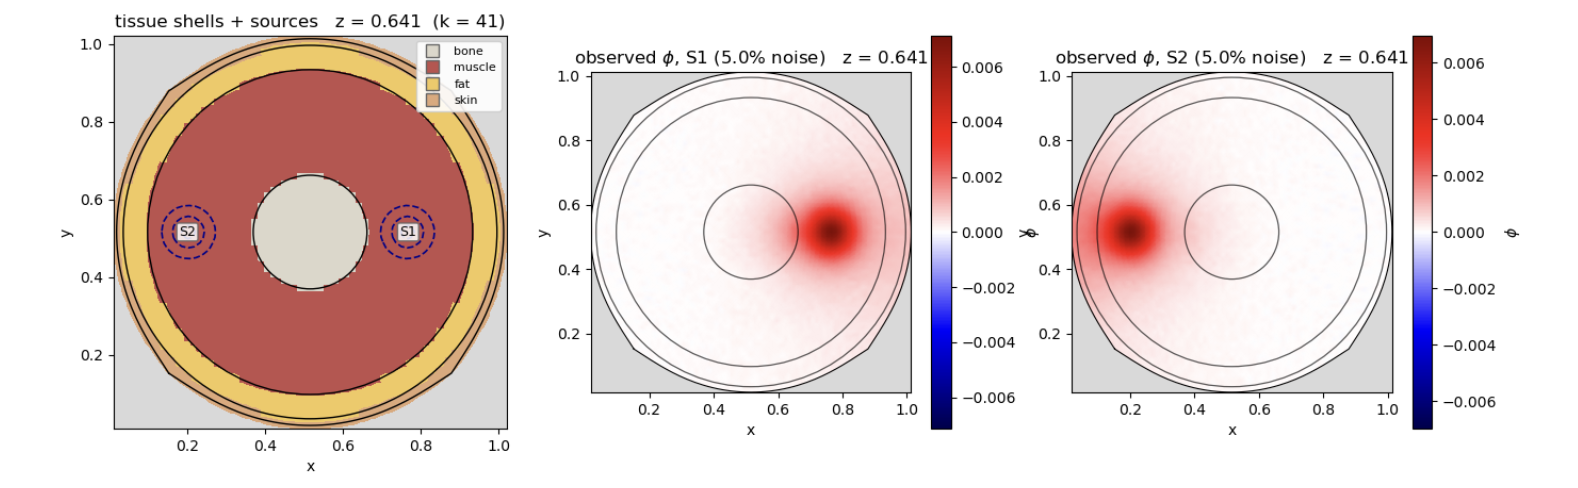
\includegraphics[width=0.8\linewidth]{experiment-design-figures/cross-section-source-visualisation.png}
  \caption{The sources and their corresponding data fields in a cross-section of the limb.}
  \label{fig:source-visualisation}
\end{figure}

The homogeneous Neumann boundary condition \ref{sec:neumann} yields the following property of the source terms, which we obtain by integrating the governing PDE over the domain $\Omega$,

$$
\begin{aligned}
\int_\Omega -I\, dV &= \int_\Omega \nabla \cdot (\sigma \nabla\phi)\, dV && \text{by the quasi-static maxwell equation} \\[2mm]
&= \oint_{\partial\Omega} \mathbf{n} \cdot (\sigma \nabla\phi)\, dS && \text{by the Divergence Theorem} \\[2mm]
&= 0 && \text{by our boundary condition} \\[2mm]
\end{aligned}
$$

For the discrete system $A\phi=b$, a solution exists if and only if $b$ lies in the range of $A$. By the Fundamental Theorem of Linear Algebra,

$$
A\phi=b \text{ has a solution}
\iff
b\in\operatorname{Range}(A)
=
\ker(A^{\mathsf T})^\perp.
$$

i.e. $b$ must lie in the orthogonal complement of the left null space of $A$. For our operator, the left null space is one-dimensional and is spanned by the trapezoidal weight vector \(W\),

$$
\ker(A^{\mathsf T})=\operatorname{span}\{W\}.
$$

Therefore, $b$ lies in $\ker(A^{\mathsf T})^\perp$ if and only if $W^{\mathsf T}b=0$.

Since $b=-I$, we have that $W^{\mathsf T}I=0$. The entries of $W$ are also the trapezoidal quadrature weights, so $W^{\mathsf T}I$ approximates $\int_\Omega I\,dV$. Thus, $W^{\mathsf T}I=0$ is the discrete analogue of the continuos net-zero current condition above.

We enforce this condition by subtracting the trapezoidal-weighted mean of the source,

$$
I_{\text{adjusted}}
=
I-
\frac{W^{\mathsf T}I}{W^{\mathsf T}\mathbf{1}}\,\mathbf{1},
$$

which ensures the discrete compatibility condition is met,

$$
W^{\mathsf T}I_{\mathrm{adjusted}}
=
W^{\mathsf T}I
-
\frac{W^{\mathsf T}I}{W^{\mathsf T}\mathbf{1}}\,
W^{\mathsf T}\mathbf{1}
= 0,
$$

where $I_{\text{adjusted}}$ is the adjusted source to ensure the system is solvable.


\section{Results}

In our experiment, we add Gaussian measurement noise to the data field $\phi$ ~\cite{vandendoel2011} to simulate noisy sEMG readings. We simulate the placement of electrodes only on the skin surface, so $\phi$ is recorded on the four lateral surfaces of our domain. At $N=65$, the surface mask contains $m=4N^2-4N=16,640$ distinct nodes per source. Since the forward map stacks the measurements from both sources, the observed data vector contains $2m=33,280$ entries:

$$
\boldsymbol{\phi}^{\mathrm{obs}}
=
\bigl[\phi_s^{\mathrm{obs}}\bigr]_{s,\mathrm{mask}}
\in\mathbb{R}^{33,280}.
$$

This represents $100$\% sampling of the lateral surfaces.

The potential fields generated by the two sources are treated as separate experiments and stacked into a single data vector. We therefore define the forward map

$$
F(\theta)
=
\begin{bmatrix}
M\phi_1(\theta)\\
M\phi_2(\theta)
\end{bmatrix}
\in\mathbb{R}^{2m}
=
\mathbb{R}^{33{,}280},
$$

where $\phi_s(\theta)$ is the potential field generated by source $s$ and $M$ selects the electrodes on the surface, which in our case is all of them. 

We choose this dense electrode coverage to simulate the placement of many electrodes because the current is not restricted to a plane, it can move freely in all three spatial dimensions above and below where the surface electrodes are placed, so the sensors should be placed on as large a surface area as possible. ~\cite{cheney1999}.

We can see the convergence of our predicted electric potential $\phi_{\text{pred}}$ towards our observed data $\phi_{\text{obs}}$, as we run iterations of our L-BFGS-B optimiser. We present five different ensemble runs with different starting values for the parameters, randomly sampled from a uniform distribution centred around their truth.

\begin{figure}[H]
  \centering
  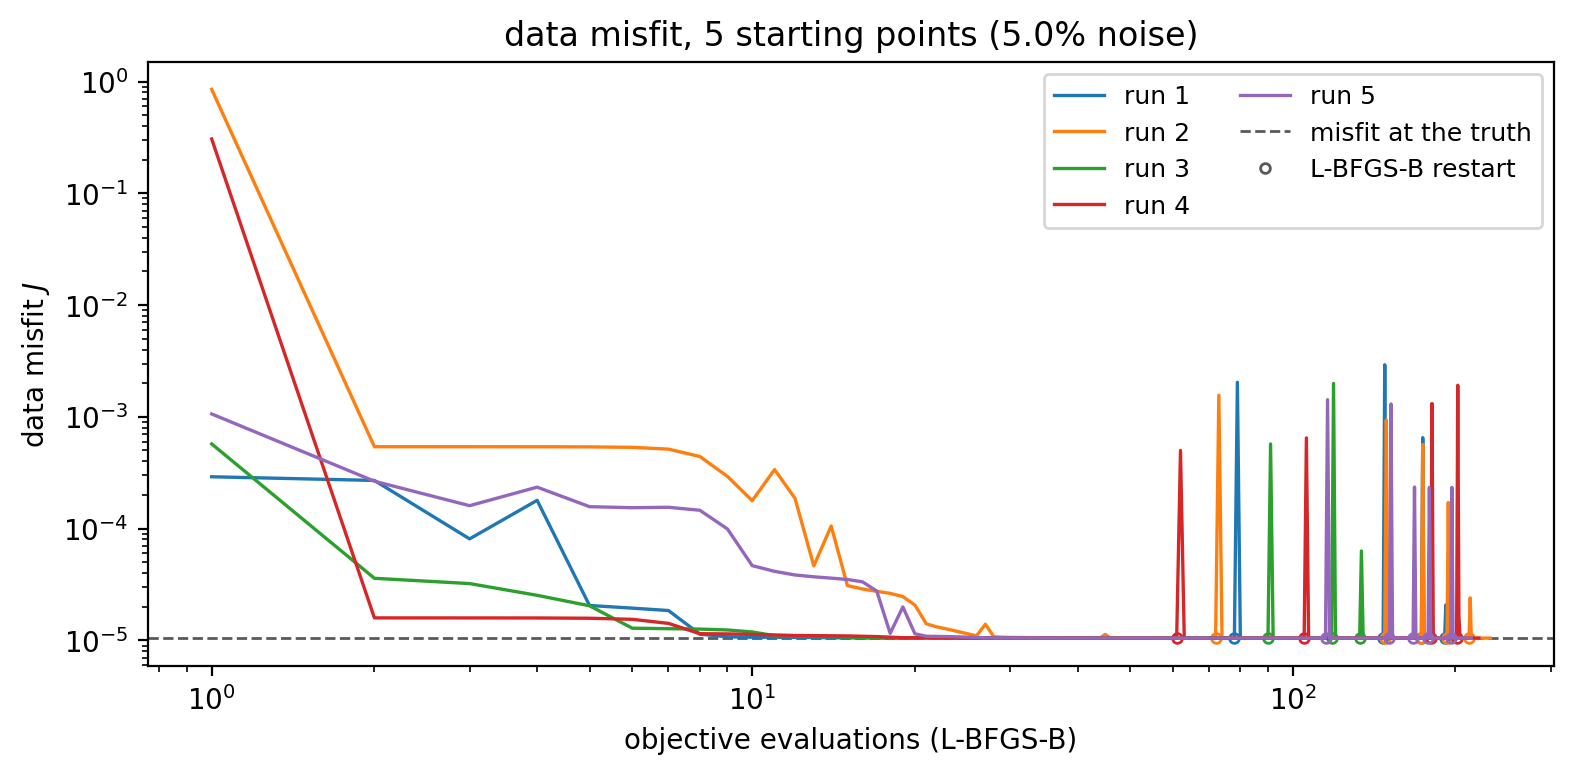
\includegraphics[width=0.8\linewidth]{experiment-results/average-data-misfit.png}
  \caption{The misfit between the predicted data field $\phi_{\text{pred}}$ and observed data field $\phi_{\text{obs}}$.}
  \label{fig:data-field-misfit}
\end{figure}

\newpage

Now we can visualise a given cross-section of the limb and watch it as it evolves through the iterations.

\begin{figure}[htbp]
  \centering
  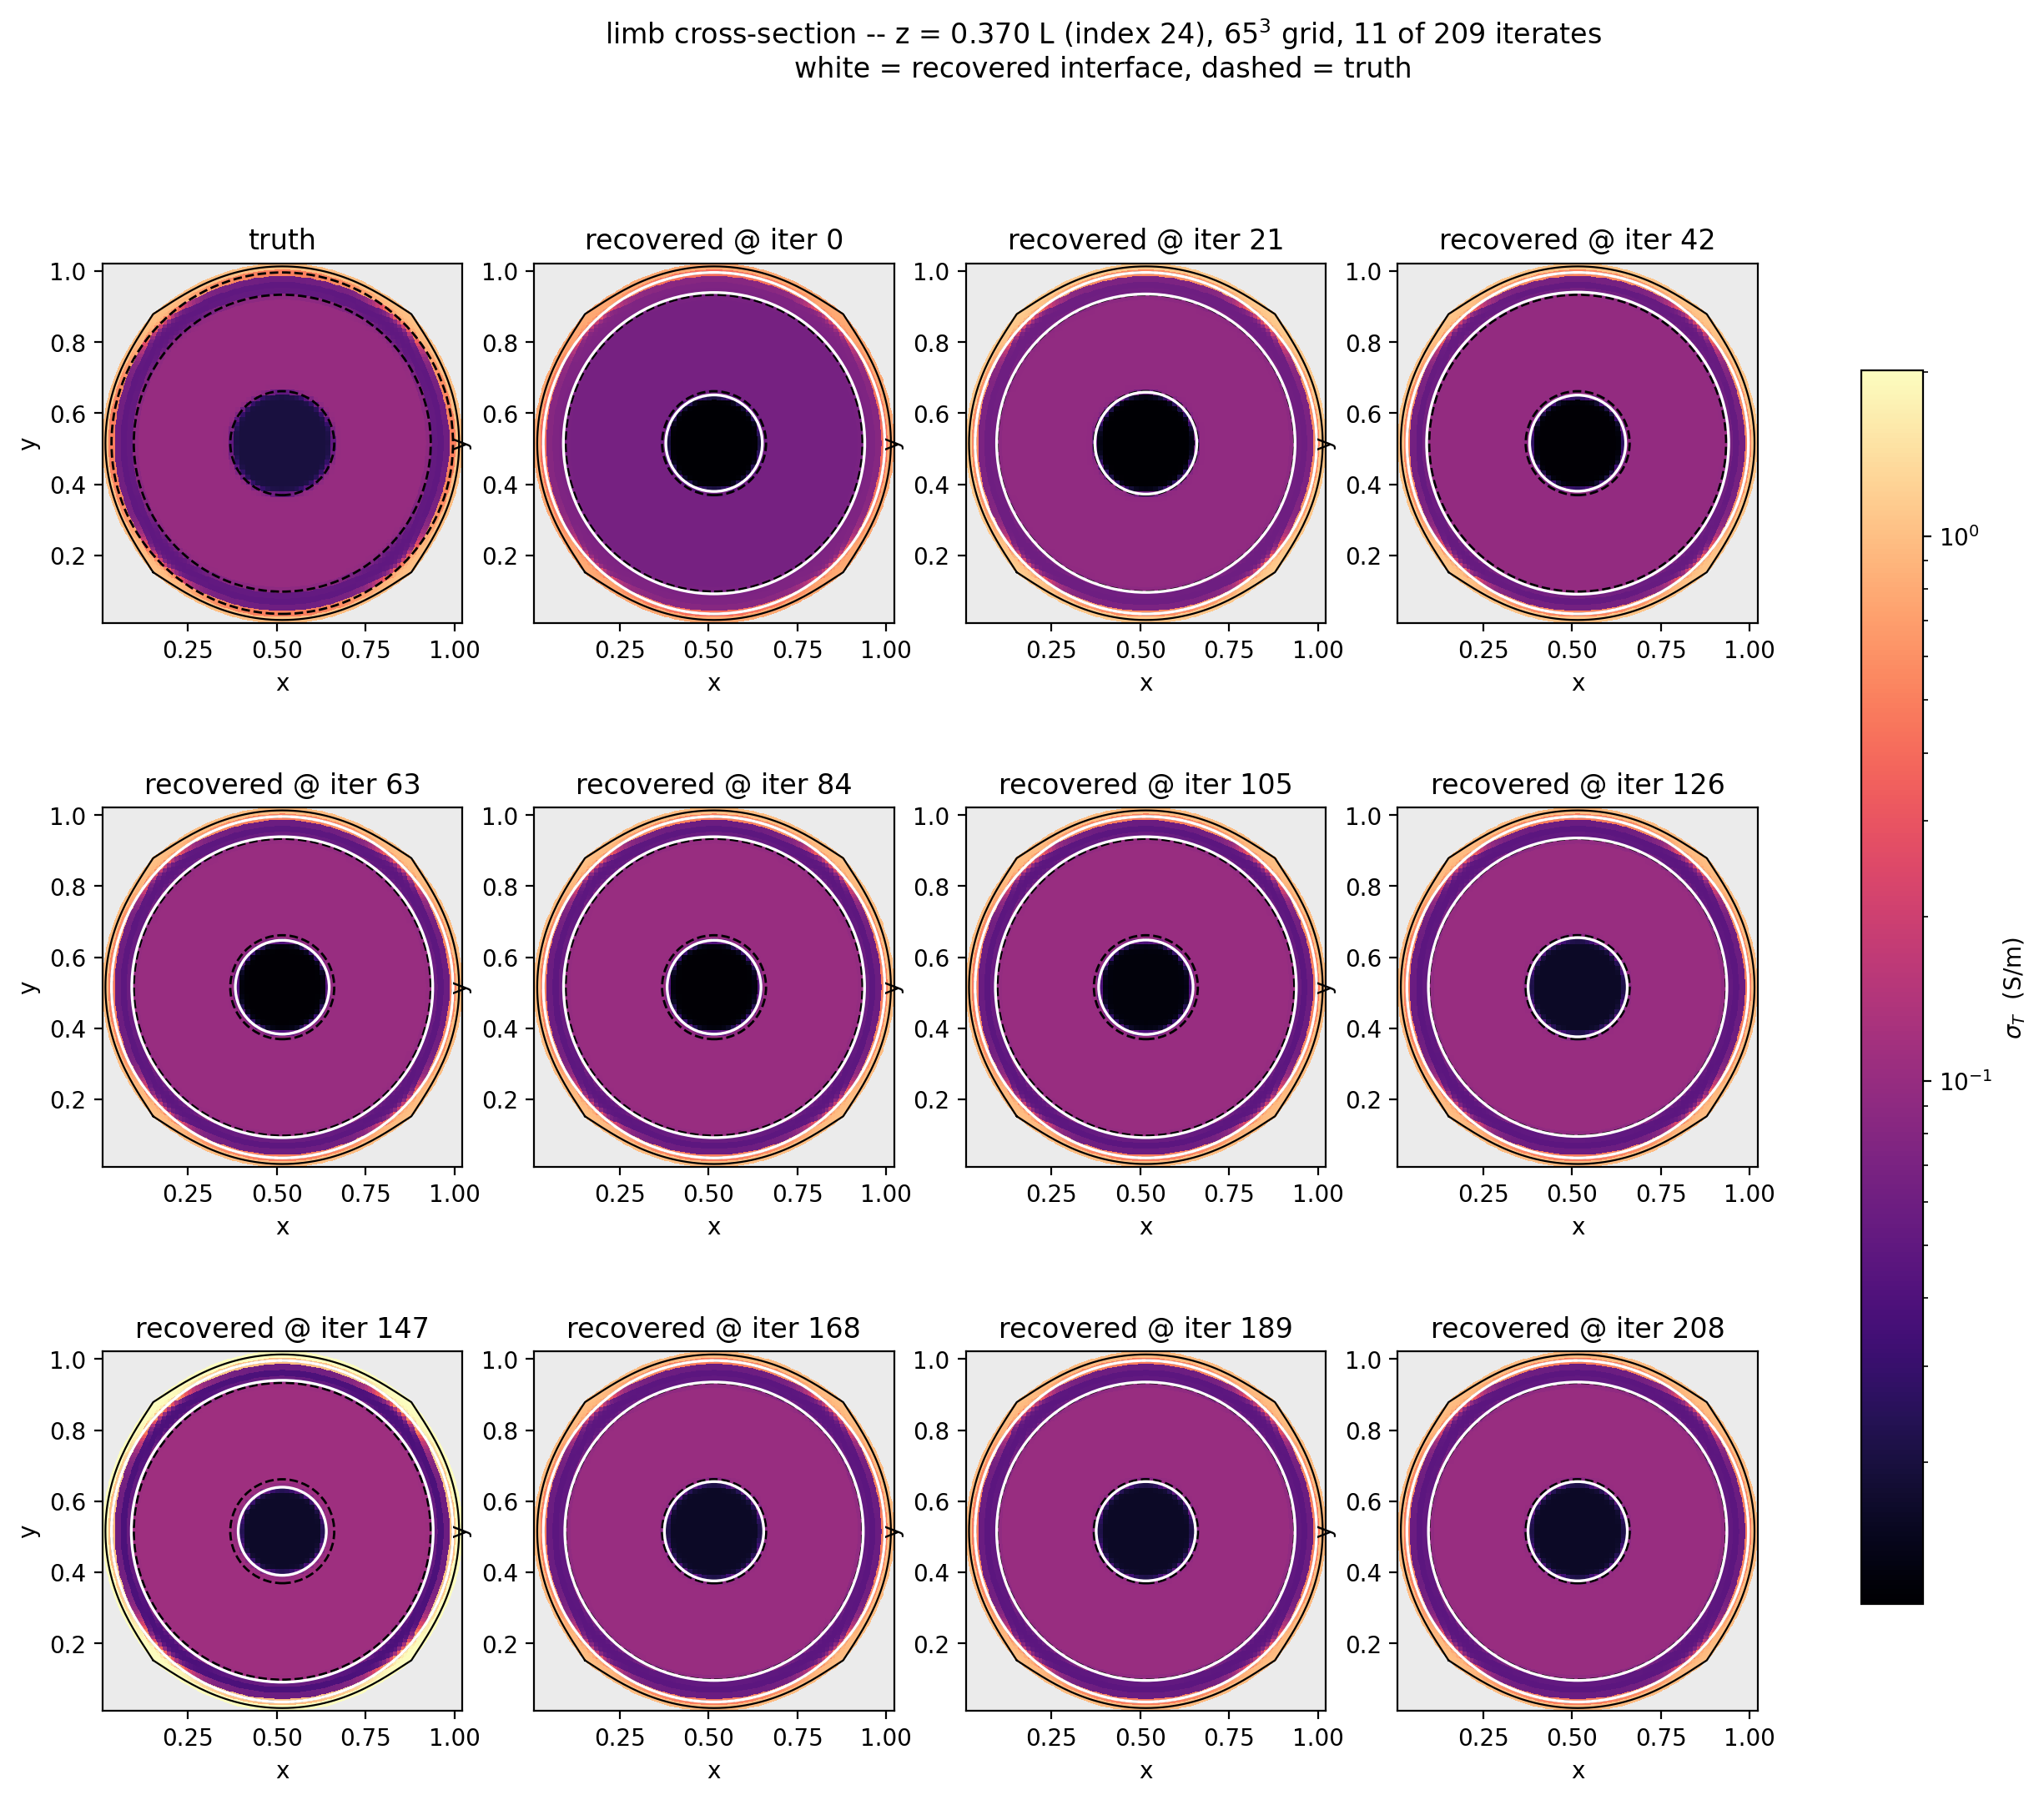
\includegraphics[width=0.8\linewidth]{experiment-results/limb-cross-section-recovery.png}
  \caption{How the cross-section of the volume conductor model changes over iterations.}
  \label{fig:layer-cross-section-evolution}
\end{figure}

We present the recovery of the seven parameters in our model, averaged over the five runs, with a measurement error of 9.3\%.

\begin{figure}[H]
  \centering
  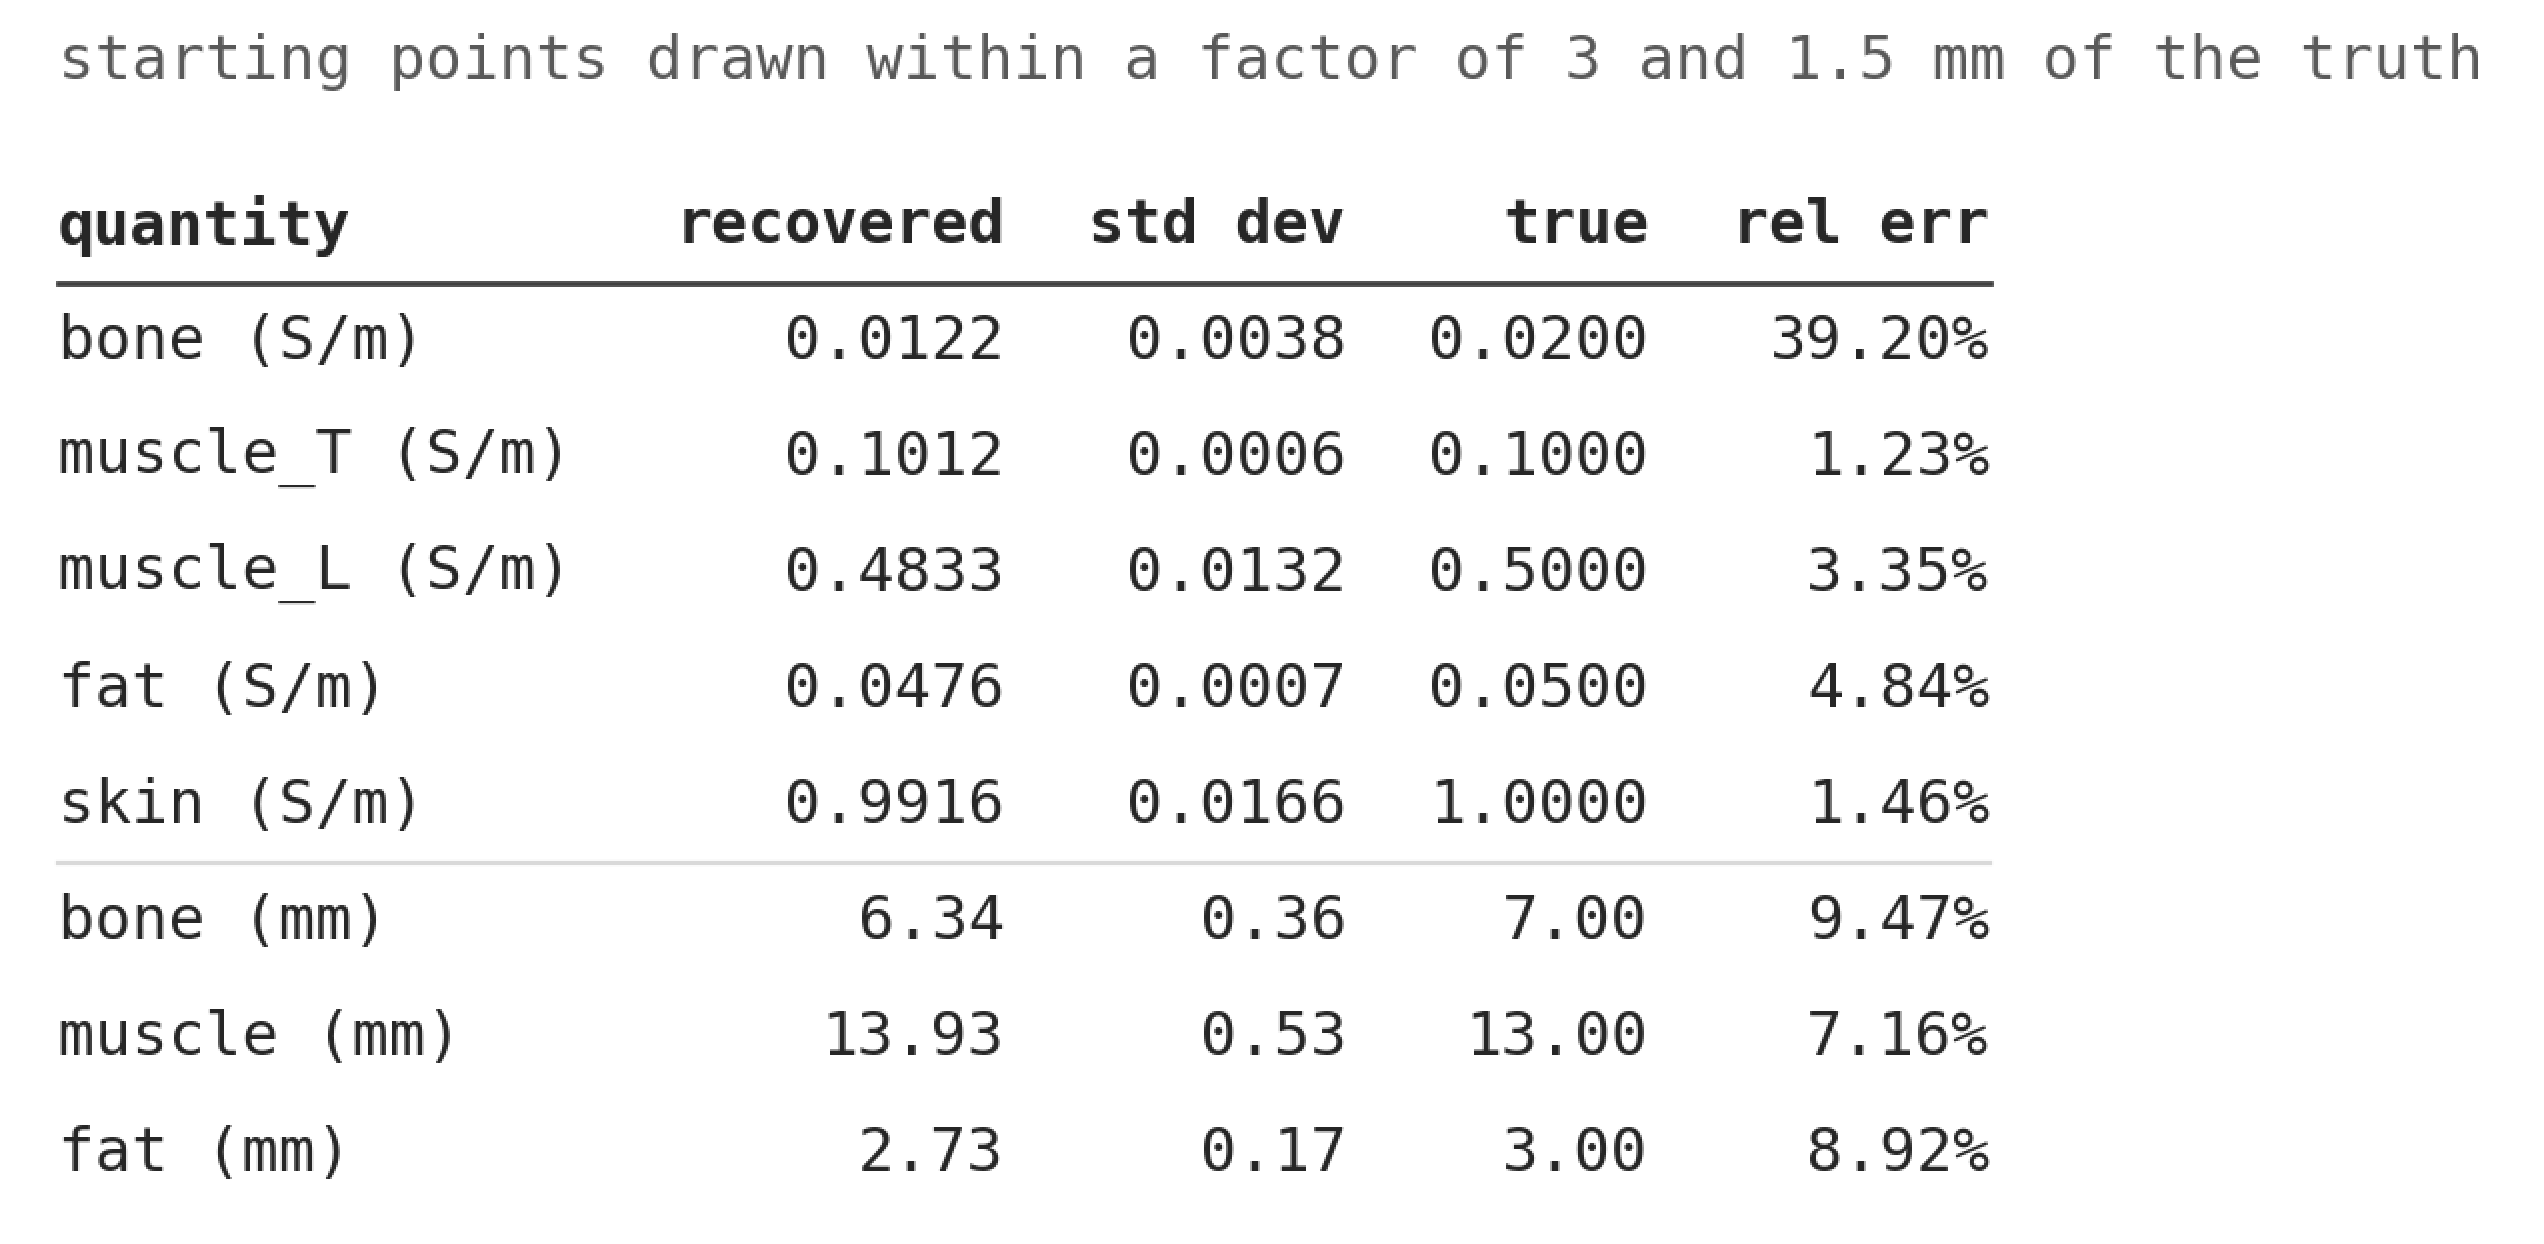
\includegraphics[width=0.8\linewidth]{experiment-results/average-parameter-recovery.png}
  \caption{Table of our parameter recoveries.}
  \label{fig:parameter-recovery}
\end{figure}

The table above reveals that the mean error in recovery of bone conductivity is significantly higher than the other parameters. Some of this is can be attributable to geometry, as bone is at the centre of the limb, so it lies the furthest from the surface electrodes.

We use the residual Jacobian $J_r: \mathbb{R}^7 \to \mathbb{R}^{33280}$ of our forward map $F$, to approximate how the forward pass responds to perturbations in the parameters. The residual vector $r(\theta) = \big[\,\phi_s(\theta) - \phi_s^{\text{obs}}\,\big]_{s,\,\text{mask}}$ i.e. the difference between predicted and measured potentials, is stacked over both the sources and restricted to the electrode nodes. We also make the entries of our parameter vector explicit, $\theta = (\theta_0, \theta_1, \theta_2, \theta_3, \theta_4, \theta_5, \theta_6) = \newline (\log\sigma_{\mathrm{bone}},\ \log\sigma_{\mathrm{muscle\_T}},\ \log\sigma_{\mathrm{muscle\_L}},\ \log\sigma_{\mathrm{fat}},\ \log\sigma_{\mathrm{skin}},\ u_0,\ u_1)$.

We perform singular value decomposition on $J_r$ to obtain information about the parameter composition of the modes in our problem.

\begin{figure}[htbp]
  \centering
  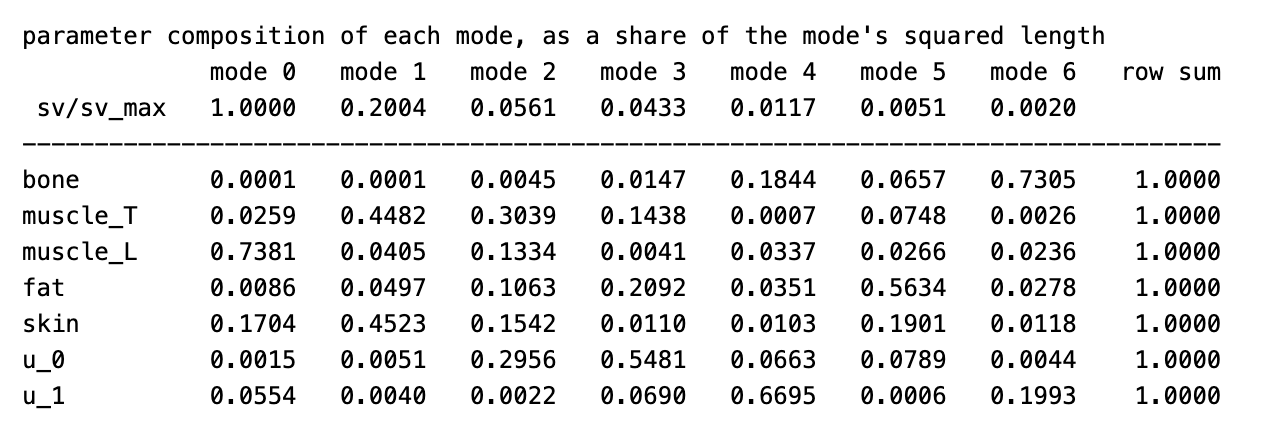
\includegraphics[width=0.8\linewidth]{experiment-results/parameter-composition-of-each-mode.png}
  \caption{Parameter composition of each mode}
  \label{fig:Mode decomposition}
\end{figure}

\begin{figure}[htbp]
  \centering
  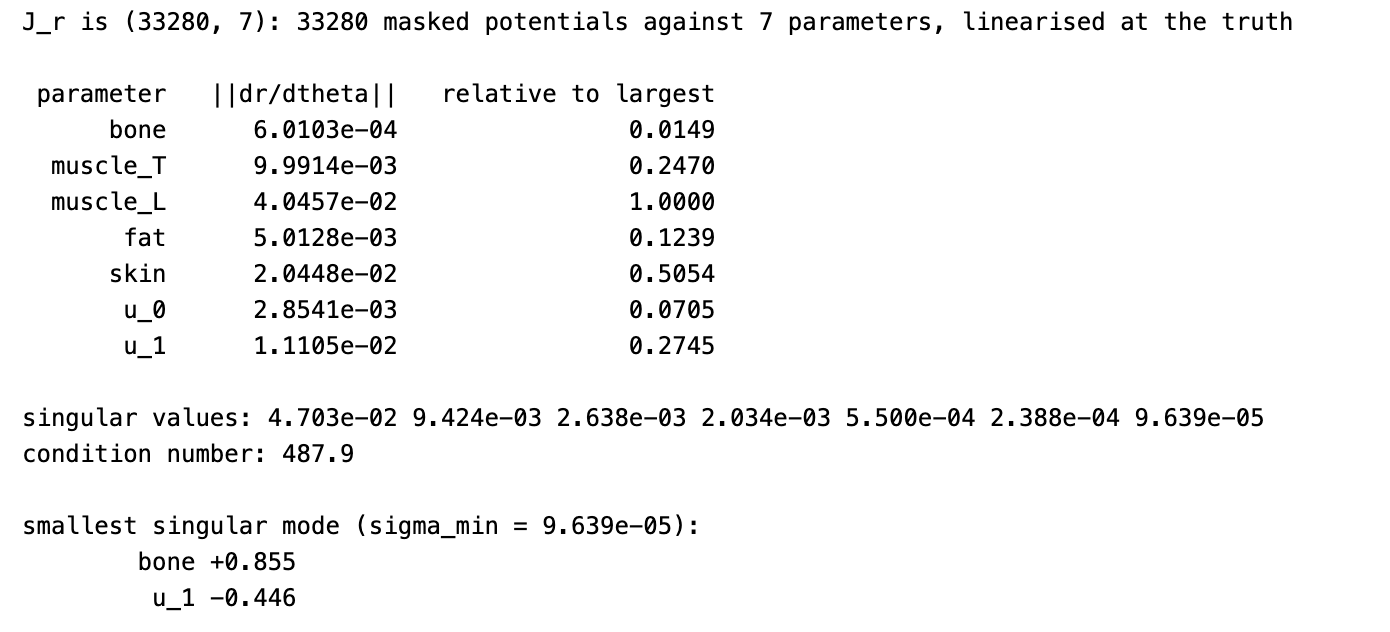
\includegraphics[width=0.8\linewidth]{experiment-results/conditioning-of-the-linearised-problem.png}
  \caption{Conditioning of the linearised problem}
  \label{fig:Conditioning}
\end{figure}

\newpage

The above figure tells our weakest singular mode is $\sigma_6 = 9.639 \times 10^-5$ and we inspect how much of the variance of the bone parameter $\theta_0$ sits inside the mode $v_6$ by performing the following variance decomposition,

$$\frac{V_{06}^2 s^2/\sigma_6^2}{\mathrm{Var}(\theta_0)} = \frac{V_{06}^2 s^2/\sigma_6^2}{\sum_{k=0}^{6} V_{0k}^2 s^2/\sigma_k^2} = \frac{V_{06}^2/\sigma_6^2}{\sum_{k=0}^{6} V_{0k}^2/\sigma_k^2} = \frac{0.7305/(9.639\times10^{-5})^2}{8.039\times10^{7}} = \frac{7.862\times10^{7}}{8.039\times10^{7}} \approx 0.978$$

So $97.8\%$ of Var($\theta_0$) lies lies in the worst resolved mode, note that the per-measurement noise variance $s^2$ cancels so this a property of the forward map only.

Turning our attention to the column norm of $\theta_0$, which is defined $\|J_r e_0\|^2 = \sum_k V_{0k}^2 \sigma_k^2$, it measures how much perturbing a given parameter, changes its residual. In Figure~\ref{fig:Conditioning}, we read that $\theta_0$ has the smallest column norm, at $1.49\%$ of the largest value. Its sensitivity is roughly 67 times lower than that of the most sensitive parameter $\theta_2$, the longitudinal conductivity in the muscle layer. This ordering is consistent with the geometry of the limb because both current sources are aligned with the longitudinal direction, so changes in $\theta_2$ have a strong effect on the measured potentials. The conductivity in the transverse direction of the muscle is also influential because it controls how much of the potential field $\phi$ moves outwards from the sources. Fat and skin surround the muscle and affect how the potentials spread towards the measurement surface, with skin having the second-largest column norm. Whereas, the bone layer is a small region in the core of the limb, away from both the sources and the measurement surface, so changes in its conductivity $\theta_0$ have a much weaker effect on the data.

Tikhonov regularisation would succeed numerically, but the bone component would still depend largely on \(\theta_{\mathrm{ref}}\), as bone is a minor contributor to the data misfit and falls almost entirely in the weakest singular mode. Even with a plausible external value of  \(\theta_{\mathrm{ref}}\), any penalty large enough to stabilise the bone component, would be prior-dominated and not data-dominated. For our synthetic experiment, constructing \(\theta_{\mathrm{ref}}\) from truth-centred initial values would introduce the further problem of using information derived from the known truth, this would make the recovery circular.

\newpage

\begin{figure}[htbp]
  \centering
  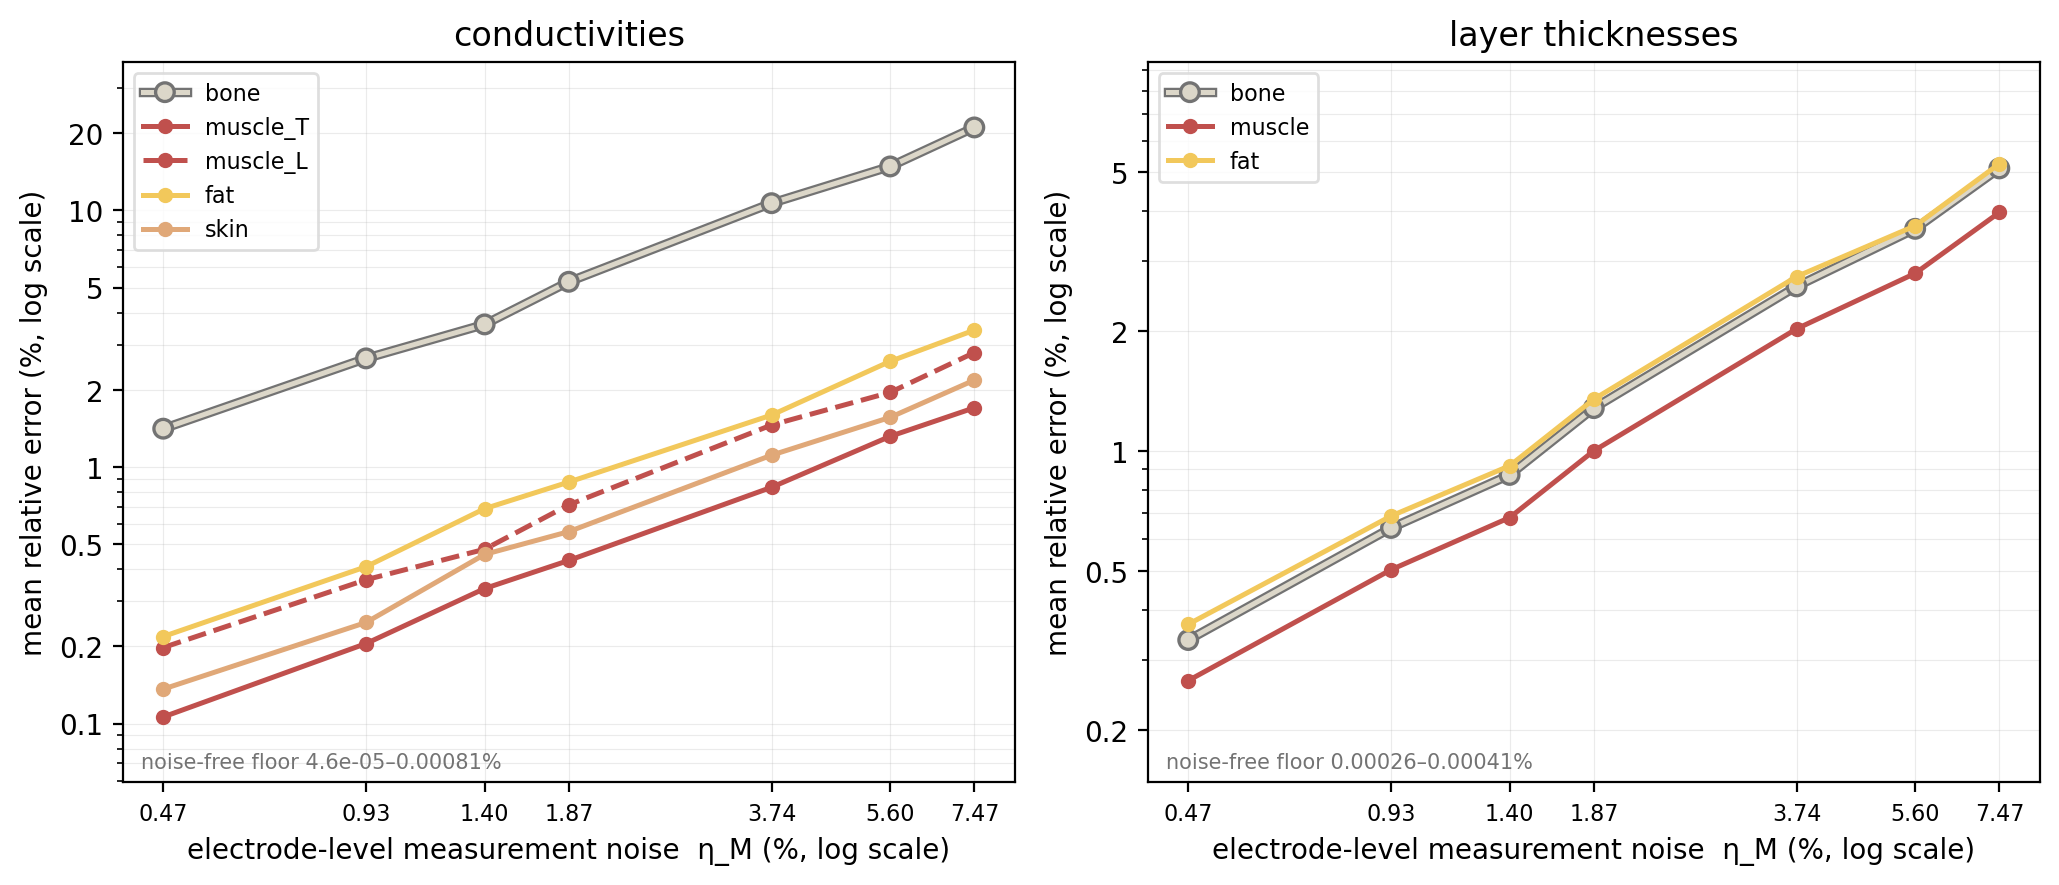
\includegraphics[width=0.8\linewidth]{experiment-results/conductivity-and-thickness-error-against-electrode-noise.png}
  \caption{Tissue conductivity and thickness recovery against noise (log-log scale)}
  \label{fig:recovery-against-noise}
\end{figure}

Our results show that even perfect noiseless data leave very small recovery errors, which range from $4.6 \times 10^{-5}\%$ to $8.1 \times 10^{-4}\%$ across the recovered quantities, due to finite discretisation errors and a fixed V-cycle budget. However, given that these errors are sufficiently small, they provide a clean floor, so the low-noise points can be interpreted against them. Figure~\ref{fig:recovery-against-noise} shows roughly straight lines with gradients that are approximately one in log-log space, this indicates that the errors scales directly proportionately with measurement noise.

Studies related to EEG source-localisation ~\cite{akalinacar2016} have found consistent conductivities for the scalp, brain and cerebrospinal fluid, however, the skull conductivity has varied massively between subjects. This provides a rough analogue for our findings, where we see that bone conductivity is much more poorly determined than the other parameters ~\ref{fig:parameter-recovery} ~\ref{fig:recovery-against-noise}.

\section{Discussion}

Results showed that the recoverability of our parameters increase as we lower the noise-floor. We conclude that bone's conductivity $\theta_0$ was poorly determined compared to the other parameters~\ref{fig:parameter-recovery}. This was expected due to it being a small region positioned at the core of the limb, so perturbing the bone conductivity causes relatively small changes in the data $\phi$, which was evidenced by $\theta_0$ having the lowest sensitivity out of all the parameters~\ref{fig:Conditioning}. In general, recovery across the board was good, as evidenced by our low mean relative errors. These results were produced by averaging over different initial starting values and the measurement noise figure\ref{fig:recovery-against-noise} over different noise seeds. We saw proportional drops in the mean relative error as we lowered the noise present at the electrodes.

Implementing our model as piecewise-homogeneous is a physical limitation because limbs consist of heterogeneous tissue, where the conductivity $\sigma(x)$ varies completely in the domain $\Omega$, so it takes distinct values for all $x \in \Omega$. Therefore, possible next steps include extending this simulation to recover the whole conductivity field $\sigma(x)$ from the voltage readings obtained from electrodes on the skin. In this setting, Neural Physics ~\cite{chen2026} becomes even more advantageous, as assigning one parameter to every grid node gives $N^3$ unknowns, where $N$ is our grid resolution, rather than the seven we recover. This would make a finite-difference Jacobian impractical. Neural Physics avoids forming the Jacobian, as it uses reverse-mode automatic differentiation to compute the gradient of the scalar data-misfit objective, with respect to all the parameters in a single backward pass. Therefore, the computational cost of the backward pass does not increase with the number of parameters.

A weakness of the proposed solution is that we do not address the inverse crime~\cite{wirgin2004}, since the same discretisation is used both for synthetic data generation and for inverse problem solution, which means the error made by the forward model is identically absorbed by the inverse process and will never appear in the residual. One way to mitigate this problem is to produce the data on a finer grid and invert on a coarser one, but this was not an option for us, as reducing the resolution means having too few nodes to be able to faithfully represent the curved rim of the limb, and therefore the discrete cross-section would become progressively more non-circular and start resembling the square it was mapped from. We would end up performing our coarse inversion on a limb with a different shape. We can address this issue by using completely different forward and inverse models, meaning that the modelling error will come from two independent sources~\cite{kaipio2007}, for example, we could generate synthetic data using a tetrahedral finite element discretisation, while performing inversion using our existing finite difference scheme.

Another limitation in our solution was related to the grid distortion. Our mapping from the square to the disc is continuous, but not continuously differentiable, thus leading to kinks at the four diagonals of the square. This introduces the error at the seams shown in figure\ref{fig:seam-error}. For future work, we could try to replace this mapping with a smooth elliptic mesh.

The most challenging aspect of this project was implementing the cylindrical grid to make our computational model honour the physical fidelity of a limb more closely. Understanding the theory this required was difficult. The handling of the homogeneous boundary conditions also presented difficulties, in regards to understanding what it would like look like to place such a requirement on the distorted grid, and the accompanying conditions that needed to be placed on the sources $I$ and the potential fields $\phi$.

\section{Acknowledgment}
I would like to offer a thank you to my supervisors Claire Heaney and Christopher Pain, who offered me regular guidance, help and ideas throughout the duration of this project.

\bibliographystyle{unsrt}
\bibliography{references} 

\appendix
%TC:ignore

\section{Mathematical Derivations}
\label{app:derivations}

\subsection{Derivation of the coordinate-transformed operator}
\label{sec:strong-form-derivation}

The identity we want is a strong-form statement i.e. the equality that must hold for every point of the domain. However, it is easier to derive the result in weak form, which involved multiplying by an arbitrary test function $\psi$ and then integrating over the domain.

We write the flux as $\mathbf F=\sigma\nabla_x\phi$, so the operator is $\nabla_x\!\cdot(\sigma\nabla_x\phi)=\nabla_x\!\cdot\mathbf F$.

Multiplying our flux by an arbitrary test function, we have via the product rule,

$$
\nabla_x\!\cdot(\psi\mathbf F)=\psi\,\nabla_x\!\cdot\mathbf F+\mathbf F\cdot\nabla_x\psi
\;\;\Longrightarrow\;\;
\psi\,\nabla_x\!\cdot\mathbf F=\nabla_x\!\cdot(\psi\mathbf F)-\mathbf F\cdot\nabla_x\psi .
$$

Integrating this over our physical domain $\Omega_x$ yields,

$$
\int_{\Omega_x}\!\psi\,\nabla_x\!\cdot\mathbf F\,dV_x
=\int_{\Omega_x}\!\nabla_x\!\cdot(\psi\mathbf F)\,dV_x
-\int_{\Omega_x}\!\mathbf F\cdot\nabla_x\psi\,dV_x .
$$

The first term on the right is the volume integral of a divergence, so we can apply the Divergence Theorem to turn it into a boundary flux,

$$
\int_{\Omega_x}\!\nabla_x\!\cdot(\psi\mathbf F)\,dV_x
=\oint_{\partial\Omega_x}\!(\psi\mathbf F)\cdot\mathbf n\,dS_x
=\oint_{\partial\Omega_x}\!\psi\, \underbrace{\mathbf F\cdot\mathbf n}_{=0},dS_x
=0
$$
where the final step holds via the homogeneous Neumann boundary condition, $(\sigma\nabla_x\phi)\cdot\mathbf n=0$, so we can drop that term from the expression.

Restoring $\mathbf F=\sigma\nabla_x\phi$ yields,

$$
\int_{\Omega_x}\!\big(\nabla_x\!\cdot(\sigma\nabla_x\phi)\big)\psi\,dV_x
= -\int_{\Omega_x}\!(\sigma\nabla_x\phi)\cdot\nabla_x\psi\,dV_x .
$$

We now perform a change of variables using $x=\Phi(\xi)$, with $dV_x=\mathcal J\,dV_\xi$ and $\nabla_x=J^{-\mathsf T}\nabla_\xi$.

The right-hand side integral of the above equation becomes,

$$
-\int_{\Omega_\xi}\!\big(\sigma J^{-\mathsf T}\nabla_\xi\phi\big)\cdot\big(J^{-\mathsf T}\nabla_\xi\psi\big)\,\mathcal J\,dV_\xi
= -\int_{\Omega_\xi}\!(\nabla_\xi\psi)^{\mathsf T}\underbrace{\big(\mathcal J\,J^{-1}\sigma J^{-\mathsf T}\big)}_{\displaystyle \tilde\sigma}\nabla_\xi\phi\;dV_\xi ,
$$

where $\tilde\sigma=\mathcal J\,J^{-1}\sigma J^{-\mathsf T}$. The dot product $\mathbf a\cdot\mathbf b=\mathbf b^{\mathsf T}\mathbf a$ is rewritten to collect the two $J^{-\mathsf T}$ factors as $J^{-1}(\cdots)J^{-\mathsf T}$.

We also push the left-hand side integral onto $\xi$-coordinates, 
$$
\int_{\Omega_x}\!\big(\nabla_x\!\cdot(\sigma\nabla_x\phi)\big)\psi\,dV_x
= \int_{\Omega_\xi}\!\big(\nabla_x\!\cdot(\sigma\nabla_x\phi)\big)\psi\,\mathcal J\,dV_\xi .
$$

So both sides are integrals against $\psi$ over $\Omega_\xi$; since they are equal for every test function $\psi$, their integrands must agree pointwise, which yields the strong-form result,

$$
\;\nabla_x\!\cdot(\sigma\nabla_x\phi)=\frac{1}{\mathcal J}\,\nabla_\xi\!\cdot(\tilde\sigma\nabla_\xi\phi)
$$

\subsection{Derivation of the transformed conductivity tensor}
\label{sec:transformed-conductivity-derivation}

The algebra holds pointwise i.e. $\sigma(x)$ does not depend on any other nodes. For our diagonal, transversely-isotropic $\sigma=\operatorname{diag}\big(\sigma_T,\sigma_T,\sigma_L\big)$, we can present it in block-form,

$$
\sigma=\begin{pmatrix}\sigma_T I_2 & 0\\ 0 & \sigma_L\end{pmatrix}.
$$

First, we deal with the in-plane (xy plane) block, where $J^{-1}\sigma J^{-\mathsf T}$ becomes $J_2^{-1}(\sigma_T I_2)J_2^{-\mathsf T}=\sigma_T\,J_2^{-1}J_2^{-\mathsf T}$. We use the inverse,

$$
J_2^{-1}=\frac{1}{\det J_2}\begin{pmatrix} d&-b\\ -c&a\end{pmatrix},
\qquad
J_2^{-\mathsf T}=\frac{1}{\det J_2}\begin{pmatrix} d&-c\\ -b&a\end{pmatrix},
$$

$$
J_2^{-1}J_2^{-\mathsf T}=\frac{1}{(\det J_2)^2}\begin{pmatrix} b^2+d^2 & -(ab+cd)\\ -(ab+cd) & a^2+c^2\end{pmatrix}.
$$

Multiplying by $\mathcal J=\det(J_2)\,z_\zeta$ gives us,

$$
M_T=\mathcal J\,J_2^{-1}J_2^{-\mathsf T}
=\frac{z_\zeta}{\det J_2}
\begin{pmatrix} b^2+d^2 & -(ab+cd)\\ -(ab+cd) & a^2+c^2 \end{pmatrix},
$$

so the in-plane part of $\tilde\sigma$ is $\sigma_T M_T$.

Now, we deal with the longitudinal block (z-axis), where $J^{-1}\sigma J^{-\mathsf T}$ in the $\zeta$-direction becomes the scalar $(z_\zeta)^{-1}\sigma_L(z_\zeta)^{-1}=\sigma_L/z_\zeta^{2}$. Multiplying by $\mathcal J=\det(J_2)\,z_\zeta$ yields,

$$
\sigma_L\,\frac{\det(J_2)\,z_\zeta}{z_\zeta^{2}}=\sigma_L\,\frac{\det J_2}{z_\zeta}=\sigma_L\,m_L,
$$

where $m_L=\frac{\det J_2}{z_\zeta}$.

Putting the blocks back together and using the matrix direct sum $\oplus$, we obtain our transformed conductivity tensor,

$$
\tilde\sigma=\sigma_T\,(M_T\oplus 0)\;+\;\sigma_L\,(0\oplus m_L)
=\begin{pmatrix}\sigma_T m_{xx}&\sigma_T m_{xy}&0\\ \sigma_T m_{xy}&\sigma_T m_{yy}&0\\ 0&0&\sigma_L m_L\end{pmatrix}.
$$


\subsection{Derivation of the harmonically averaged face coefficients}
\label{sec:averaging-face-coefficients}

The flux form needs a coefficient at $x_{i+\frac12}$, but $a$ is stored at the
nodes. Therefore, we construct a face value $a_{i+\frac12}$ via averaging, which must be the number for which the two-point difference reproduces the flux between $\phi_i$ and $\phi_{i+1}$. Note that $x$ is a continuos variable and $a_i = a(x_i)$ are discrete samples of it.

Since the diagonal term is a two-point flux along a single axis, the derivation is given for one and applies similarly for the other two axes. We have that on $[x_i,x_{i+1}]$ the flux $F=-a\phi'$ is constant, so $\phi'=-F/a$ and
\[
  \phi_{i+1}-\phi_i \;=\; -F\!\int_{x_i}^{x_{i+1}}\!\frac{1}{a(x)}\mathrm{d}x,
  \qquad\text{giving}\qquad
  a^{\star}_{i+\frac12}
  \;=\; h\left(\int_{x_i}^{x_{i+1}}\!\frac{1}{a(x)}\mathrm{d}x\right)^{\!-1}.
\]
The derivation assumes only that $a$ is positive and integrable and makes no assumption about the continuity of $a$. We evaluate the integral via the trapezoidal rule,
$\int \frac{1}{a(x)}\mathrm{d}x\approx\tfrac{h}{2}(a_i^{-1}+a_{i+1}^{-1})$, which gives
\[
  a^{\star}_{i+\frac12}\;\approx\;\frac{2a_ia_{i+1}}{a_i+a_{i+1}}
  \;=\;\operatorname{harm}(a_i,a_{i+1}).
\]

The cross coefficient $m_{xy}$ is the only face coefficient that is excluded from this because it admits no two-point
face flux and it is sign-indefinite, and the harmonic mean is not defined for sign-indefinite quantities. Thus, it is handled separately in Section~\ref{sec:cross-term}.

\subsection{Derivation of the cross-term}
\label{sec:cross-term}
To discretise the cross term, we multiply the PDE by a test field \(\psi\) and integrate by parts. The boundary contribution vanishes because \(\tilde{\sigma}\nabla_\xi\phi\cdot\mathbf N=0\), leaving

$$
\int_\Omega \psi\,\nabla_\xi\!\cdot\!\big(\tilde{\sigma}\nabla_\xi\phi\big)\,\mathrm dV_\xi
=
-\int_\Omega
\big(\nabla_\xi\psi\big)^{\mathsf T}
\tilde{\sigma}\nabla_\xi\phi\,\mathrm dV_\xi.
$$

The full derivation of this is handled in appendix~\ref{sec:strong-form-derivation}. We expand the in-plane block $\sigma_T M_T$ to give,

$$
\big(\nabla_\xi\psi\big)^{\mathsf T} \big(\sigma_T M_T\big)\nabla_\xi\phi = \sigma_T\left[ m_{xx}\phi_\xi\psi_\xi +m_{yy}\phi_\eta\psi_\eta +m_{xy}\big(\phi_\xi\psi_\eta+\phi_\eta\psi_\xi\big) \right].
$$

The first two terms are the already assembled diagonal fluxes~\ref{sec:operator-discretisation}, so the cross-term contribution is,

$$
b(\phi,\psi) = -\int_\Omega \sigma_Tm_{xy} \big(\phi_\xi\psi_\eta+\phi_\eta\psi_\xi\big) \,\mathrm dV_\xi.
$$

We approximate this integral by using the midpoint rule on every in-plane cell $c=[\xi_i,\xi_{i+1}]\times[\eta_j,\eta_{j+1}]$ (each cell consists of four nodes). The values of $\phi$, $\psi$, $\sigma_T$, and $m_{xy}$ are stored at the four corner nodes of the cell.

We approximate the derivative of $\phi$ in the following manner,

$$
(\phi_\xi)_c = \frac{\big(\phi_{i+1,j} - \phi_{i,j}\big) + \big(\phi_{i+1,j+1}-\phi_{i,j+1}\big)}{2h},
$$

$$
(\phi_\eta)_c = \frac{\big(\phi_{i,j+1}-\phi_{i,j}\big) + \big(\phi_{i+1,j+1}-\phi_{i+1,j}\big)}{2h}.
$$

The derivatives of $\psi$ are calculated in the same way. The coefficient at the midpoint $\sigma_Tm_{xy}$, is approximated by the arithmetic mean of the four corner values of the product,

$$
\big(\sigma_Tm_{xy}\big)_c
=
\frac14\left[
\big(\sigma_Tm_{xy}\big)_{i,j}
+\big(\sigma_Tm_{xy}\big)_{i+1,j}
+\big(\sigma_Tm_{xy}\big)_{i,j+1}
+\big(\sigma_Tm_{xy}\big)_{i+1,j+1}
\right].
$$

At a fixed \(\zeta\)-level, the midpoint rule gives,

$$
b_h^{(k)}(\phi,\psi) = -h^2\sum_c \big(\sigma_Tm_{xy}\big)_c \left[ (\phi_\xi)_c(\psi_\eta)_c + (\phi_\eta)_c(\psi_\xi)_c \right],
$$

where \(h^2\) is the area of each in-plane cell. These contributions are then summed over the \(\zeta\)-levels, which supplies the remaining factor of $h$ in the 3D integral.

%TC:endignore
\end{document}